
% Template PNSAC newsletter - Article
% Language: Latex
%

% Head

\title{Project Manager's Progress Report}
\subtitle{April 2013}
\author{Bruce Gemmill}

\maketitle

During the last three months we have continued working on our two top
priorities -- Engine \#3 and the interior of the North Star.  Some of
the external skin has also been polished.  Volunteers were also
involved in preparing the North Star and Argus for an early move
outside, to accommodate an exhibit in the Storage Wing.

\section{Engine and QEC}
\label{sec:engines}

The engine rebuild is nearing completion, with magnetos and a few
other accessories to be installed.  The completed engine will soon be
installed in the engine frame, then work will begin on the
supercharger and intercooler.

\begin{figure}[htbp]
   \vspace{2em}
   \centering
   %name of the graphic, without the path AND in EPS format:
   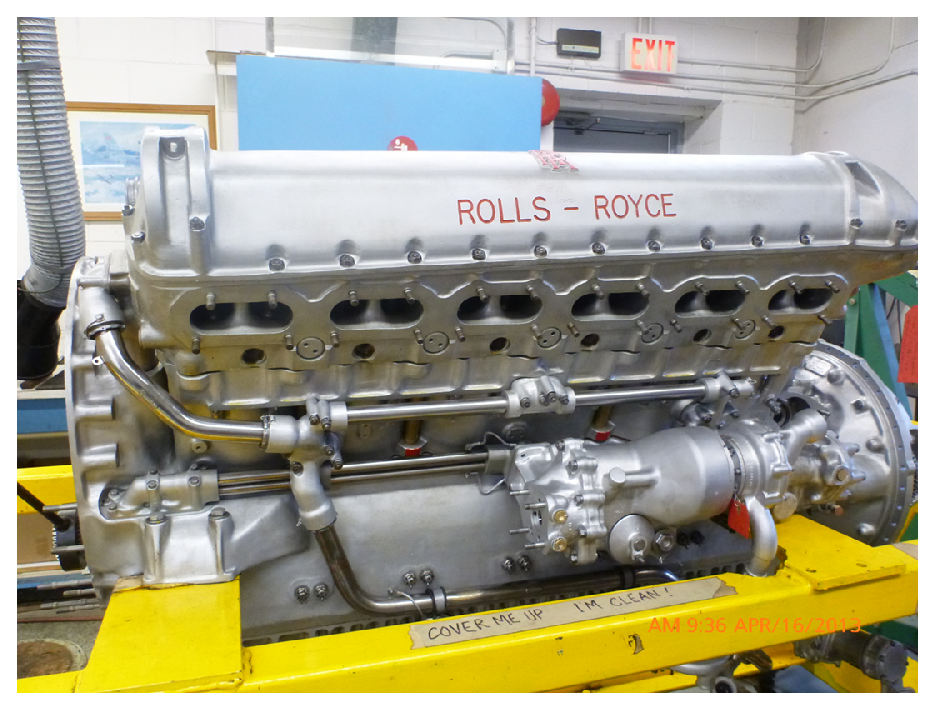
\includegraphics[scale=0.5]{engine3.eps}
   %caption of the figure 
   \caption*{\small \em North Star engine 3.}
   %label of the figure, which has to correspond to \ref{}:
   \label{fig:engine3}
\end{figure}


The basic engine frame is back together.  The three radiator sections
were cleaned and painted, then attached to the front of the frame.
The rear cowl ring has been disassembled, and new mounting hardware is
being fitted before the parts are painted and reassembled.  The front
cowl assembly (radiator cover) has also been cleaned, repaired and
polished, ready to install.  Other cowl panels will each be cleaned,
repaired and polished, ready to install once the complete engine is in
place.  Work is also underway on a host of pipes, cables, accessories
and fittings needed to complete the assembly of the engine and QEC
prior to installation on the aircraft.

As mentioned, volunteers worked to prepare the North Star for an early
move outside.  Besides installing windows and closing other openings
for weather protection, propeller \#2 was installed on engine \#2,
rather than keeping it stored in the hangar.

\section{Fuselage and Crew Area}
\label{empennage}

The crew lounge and forward washroom are looking more finished,
although much work still remains.  New Plexiglas windows were
installed in the crew lounge, washroom and APU closet.  The water tank
was installed in the ceiling, and the water lines hooked to the newly
refurbished sink. 
 
The air scoop that supplied cold air to the Janitrol heaters was badly
corroded and removed for repair.  This involved cutting away damaged
aluminum and riveting carefully formed patches in place.  The assembly
was primed, then riveted back in place over the crew lounge.  New
insulation was installed in the ceiling, including a layer of heat
resistant mica.  Some pipes and wires have been installed, and the
heating ducts were cleaned and recovered with fabric.  These will be
installed once the Janitrol heaters are in place.

The new galley is almost complete.  After the original doors are
repaired they will be attached to the new assembly, which can then be
installed in the crew lounge, just behind the equipment rack.  New
wiring legends were produced for the inside of the electrical
cabinets.  These will be laminated before installation, to prevent
deterioration from humidity.

The ceiling and wall panels in the forward and rear belly compartments
have been stencilled and installed.  The floor panels were badly
scratched and in some cases stretched, due to the heavy load of
baggage often carried in these compartments.  Each panel is being
assessed, and several have already been remade.  These will be painted
and stencilled, then installed later this spring.

One of the new de-icing boots has been successfully manufactured.
This will be an on-going project, as time permits.  Completed boots
will be stored until other repair work on wings and stabilizers has
been completed.

Work has begun manufacturing a full set of troop seats for the
aircraft.  A total of 33 seats will be sewn and fitted to new mounting
frames.  A design has been completed and fabric work has started.
Some of the fittings have also been made.  This work will continue for
some time and all completed items will be stored until the main cabin
has been repainted. 


\begin{figure}[htbp]
   \vspace{2em}
   \centering
   %name of the graphic, without the path AND in EPS format:
   \includegraphics[scale=0.5]{sink_vanity.eps}
   %caption of the figure 
   \caption*{\small \em Forward vanity.}
   %label of the figure, which has to correspond to \ref{}:
   \label{fig:vanity}
\end{figure}

The forward washroom has most equipment returned, including the toilet
and the window, minus the Plexiglas insert that is on order.
Likewise, the vanity mirror and various fixtures were repainted and
re-installed.  The door will not be installed until the new flooring
is glued down, one of the last tasks in the crew area.

The APU compartment, which had been converted to luggage and coat
storage, has been re-assembled.  The power inverter and cabinet were
re-installed, along with the luggage shelf and floor.

% The heater and ducting has become a major item of work.  All the ducts
% were removed and cleaned, but new woven fibreglass coverings will need
% to be attached.  Material is on order.  The main air scoop that feeds
% the heater was removed and found to be badly corroded.  This item is
% being rebuilt and must be installed before the aircraft goes outside
% this spring.

% Work also continues on the floor, ceiling and wall panels from the
% under floor belly compartment.  Some damaged panels may need to be
% replaced.  Progress is also being made on the de-icing boots for the
% wings

% We made good progress on our plan to build a set of troop seats for
% the aircraft.  Our appeal for donations was highly successful, and
% most of the material needed for the seats has now been received.
% Numerous fittings were manufactured and painted, and are stored until
% the seats are ready to install. 

\section{Planned Restoration Work--2013}
\label{sec:plannedwork}

This summer we will replace all the items removed from the crew areas
and continue the rebuild of engine \#3.

Sewing of the seat fabric will begin soon and will continue until all
the fabric has been stitched together.  The frames will be
manufactured later this year

Next we expect to begin work to restore the main cabin.  This will
require removal of the wood cargo floor for a thorough cleaning and
inspection.  We expect to find some corrosion damage that will require
repair. 


%% \begin{figure}[htbp]
%%    \vspace{2em}
%%    \centering
%%    %name of the graphic, without the path AND in EPS format:
%%    \includegraphics[scale=0.5]{MerlinCylinderHead.eps}
%%    %caption of the figure 
%%    \caption*{Richard Lodge and Garry Dupont, Merlin Cylinder Head}
%%    %label of the figure, which has to correspond to \ref{}:
%%    \label{fig:eng_one}
%% \end{figure}

\begin{footnotesize}
  \raggedleft PNSAC\\
\end{footnotesize}

% End of text.

%%% Local Variables: 
%%% mode: latex
%%% TeX-master: main_document.tex
%%% End: 

